\chapter{Методология и архитектура}
\label{chap:met}

\section{Интеграция копилятора}
\label{sec:met:ls_compiler_interop}
Идея Языкового Сервера заключается в том, чтобы запускать экземпляр ЯС в том же каталоге проекта, который открыт в редакторе, и в подключении его к редактору по протоколу ЯС.

Языковой сервер отвечает за реализацию функций редактора по работе с кодом, он оперирует над семантическим представлением языка и другими метаданными, 
нужными для осуществения семантического анализа и, следовательно, предоставляет редактору данные в согласованном формате через протокол языкового сервера. 
Поскольку языковой сервер в значительной степени полагается на современный компилятор, который предоставляет SR, 
нам нужно реализовать способ интеграции компилятора в языковой сервер и обеспечить их взаимодействие.

Это можно сделать двумя способами: либо использовать компилятор в качестве библиотеки, 
либо вызывать его в отдельном процессе, передавая компилятору требуемые аргументы командной строки.\ref{table:met:compiler_integration}
\begin{table}[H]
    \centering
    \begin{tabular}{|c|c|}
        \hline
        \textbf{вызов команды} & \textbf{подключение через API} \\
        \hline
        \makecell{более простая интеграция} & \makecell{сложная интеграция} \\
        \hline
        \makecell{ограниченное количество опций вызова} & \makecell{возможность выражать сложные \\стратегии интеграции} \\
        \hline
        \makecell{необходисомть в разборе формата} & \makecell{возможность обмениваться \\типами данных компилятора} \\
        \hline
        \makecell{необходимость реализации своего \\API обхода семантического представления} & \makecell{компилятор может экспортировать \\API обхода представления} \\
        \hline
        \makecell{необходимость описания типов данных \\компилятора в языковом сервере} & \makecell{компилятор может экспортировать \\внутренние типы данных} \\
        \hline
    \end{tabular}
    \caption{Сравнение методик интеграции компилятора в языковой сервер}
    \label{table:met:compiler_integration}
\end{table}

Поскольку компилятор SLang\cite{Zouev2017} не предоставляет API обхода AST или внутренних типов данных, большинство преимуществ, 
характерных для опции "подключение через API", не применимы в нашем случае. 
Кроме того, компилятор предоставляет стабильное семантическое представление в формате JSON, который, 
будучи стандартизированным текстомым форматом, может быть легко передан через канал операционной системы, такой как standard output\cite{TheOpenGroup1997}.

Таким образом, мы получаем ряд удобных свойств когда компилятор вызывается нашим языковым сервером как команда, к тому же
этот вариант легче реализовать как на стороне языкового сервера, так и на стороне компилятора. 
И поскольку мы не ограничены какой-либо функциональностью, которая требовала бы подключения компилятора через API, 
мы можем считать этот способ интеграции наиболее уместным в нашем случае и придерживаться его.\ref{fig:met:compiler_integration}
\begin{figure}[H]
    \centering
    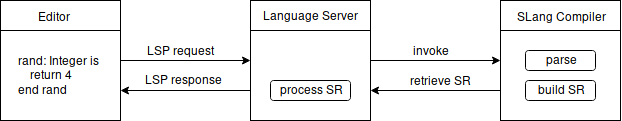
\includegraphics[width=1.0\textwidth]{figs/compiler_integration.png}
    \caption{Взаимодейёствие компилятора с языкомым сервером}
    \label{fig:met:compiler_integration}
\end{figure}

\section{Расширяемая архитектура языкового сервера}
\label{sec:met:arch}
Основная идея данного исследования состоит в подъеме архитектуры языковых серверов на новый уровень, сделав их модульными и расширяемыми, таким образом позволив третьим лицам добавлять свой функционал в инструментарий SLang, без необходимости разбираться в коде самого языкового сервера и вносить туда изменения.
Соответственно, архитектура языкового сервера SLang разделена на два связанных компонента: \ref{fig:met:ls_highlevel_arch}
\begin{itemize}
    \item Ядро
    \item Модульная система
\end{itemize}

\begin{figure}[H]
    \centering
    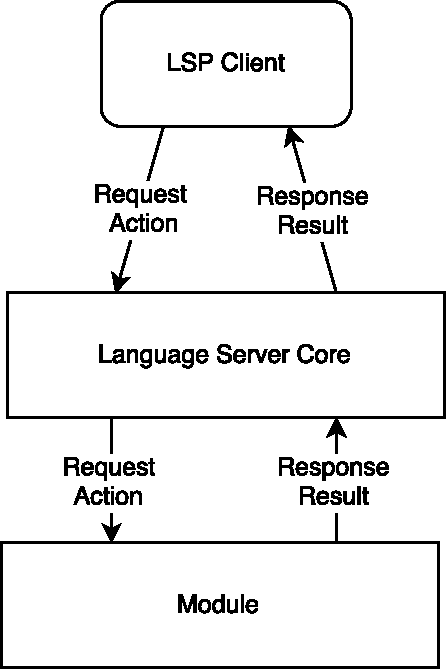
\includegraphics[width=.3\textwidth]{figs/highlevel_architecture.pdf}
    \caption{Высокоуровневая архитектура языкового сервера}
    \label{fig:met:ls_highlevel_arch}
\end{figure}

\subsection{Ядро языкового сервера}
\label{sec:met:arch:core}
Ядро языкового сервера --- это основание языкового сервера, поверх которого наложено фунционирование модулей языкового сервера. Ядро ЯС должно отвечать за:
\begin{itemize}
    \item поддержку соединения клиента ЯС
    \item Поддержку реестра модулей
    \item Распределение входящих запросов и контроль потока данных между модулями
\end{itemize}

Ниже будет описана каждая из этих зон ответственности.

\subsubsection{ПОддержка соединения с клиентом}
\label{sec:met:arch:core:connection_maintenance}
Согласно протоколу языкового сервера\cite{Sourcegraph}, клиент контролирует время жизни сервера, т.е запускает и выключает его по мере необходимости. После запуска, клиент подключается к серверу одним из доступных путей. Поскольку транспортный уровень не ограничен LSP, различные реализации могут позволять различный транспорт.

Ядро языкового сервера должно поддерживать несколько разновидностей транспорта и быть способно использовать их для принятия запросов иотправки ответов клиенту. Мы собираемся реализовать следующие из них:
\begin{itemize}
    \item stdin/stdout
    \item TCP
    \item UDP
\end{itemize}
Реализация пунктов данного списка позволит обеспечить большинству клиентов LSP выбор способа работы с языковым сервером SLang.

\subsubsection{Реестр модулей}
\label{sec:met:arch:core:module_registry}

Чтобы быть основой для расширяемой модульной архитектуры, ядро языкового сервера должно включать в себя подсистему для регистрации, поддержки, и организации взаимодействия модулей.

\begin{figure}[H]
    \centering
    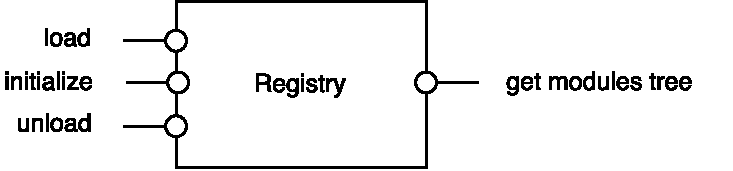
\includegraphics[width=.7\textwidth]{figs/registry.pdf}
    \caption{API реестра модулей}
    \label{fig:met:registry_methods}
\end{figure}

\newpage
Реестр должен регистрировать модуль и публиковать его статус, а также информацию о способах запуска и соединения ядра с внешними модулями. При запуске, реестр должен инициализироваться, используя предопределенную директорию, содержащую файлы конфигурации. После этого он должен поддерживать API для загрузки и выгрузки добавочных модулей через LSP. Впоследствии нам потребуется расширить LSP добавочными командами для реестра модулей:\ref{fig:met:registry_methods}

\begin{itemize}
    \item registryCtl/load: зарегистрировать модуль.
    \item registryCtl/unload: разрегистрировать модуль.
    \item registryCtl/status: узнать статус модуля.
\end{itemize}

\subsubsection{Диспетчер и контроль потока данных}
\label{sec:met:arch:core:dispatcher}
После запуска, установления соединения, регистрации модулей и инициализации, языковой сервер может принять первый запрос от клиента. Этот запрос валидируется ядром языкового сервера, и затем, после просмотра реестра модулей, запрос передается в начало процесса обработки запроса, ответственного за данный тип запросов.

Диспетчер по факту является связующим элементом, соединяющим вместе все компоненты языкового сервера и поддерживающим ребра потока данных на графе модулей, позволяя взаимодействие модулей по правилам, загруженным в реестр, которые расписаны подробнее в секции \ref{sec:met:arch:ms}

Существует более простой альтернативный подход к организации взаимодействия модулей: позволить модулям обмениваться данными друг с другом и организовывать последовательность действий по собственному разумению. Хотя данная пиринговая схема позволила бы требовать меньшую пропускную способность, она также неизбежно приведет к возникновению сложноподдерживаемого графа зависимостей, поскольку данный подход потребовал бы, чтобы все модули знали друг о друге и были соединены друг с другом. Таким образом, здесь мы имеет традиционный конфликт между эффективностью сервера и эффективностью клиента: мы можем разгрузить ``сервер'' (ядро ЯС) только посредством усложнения ``клиента'' (модулей). Поскольку клиентская сторона в данном случае предположительно будет разрабатываться третьими лицами, чем проще она --- тем лучше: сервер будет контролировать поток данных, что позволит разработчикам сосредоточиться на логике модуля.

\subsection{Система модулей}
\label{sec:met:arch:ms}

Языковой сервер --- прекрасная идея, наделяющая сравнительно простые текстовые редакторы функционалом уровня IDE, однако в наше время они проектируются монолитными, в то время как их функционал естественным образом предполагает расширяемость, например, очень часто статический анализатор будет также иметь несколько модулей для диагностики, что подразумевает иерархию как минимум двух модулей --- диагностики компилятора и диагностики с помощью стороннего инструмента статического анализа. Можно пойти еще дальше и реализовать статический анализатор как комбинацию базового модуля статического анализа и множества атомарных диагностических модулей, отнаследованных от базового модуля. Подобная логика в той или иной мере применима к любому сервису языкового сервера.

Отделение монолитного ядра от фактического функционала, реализованного через модули значительно снизит внутреннюю связность языкового сервера, что позволит реализацию модулей, основанных на максимально надежном API, и соответственно, одновременную разработку ядра и модулей без случаев взаимного разрушения API.

Соответственно, другое полезное следствие расширяемой архитектуры состоит в том, что языковой сервер может быть легко приспособлен под любые специфические корпоративные нужды. Поскольку реализация дополнительного функционала будет так же проста, как разработка плагина с помощью API модулей языкового сервера, корпоративные пользователи могут расширить языковой сервер в соответствии со своими конкретными требованиями, например, добавив свою собственную диагностику, принятое форматирование кода, или даже прикрутив проприетарные статические анализаторы или инструменты для генерации кода.

\begin{figure}[H]
    \centering
    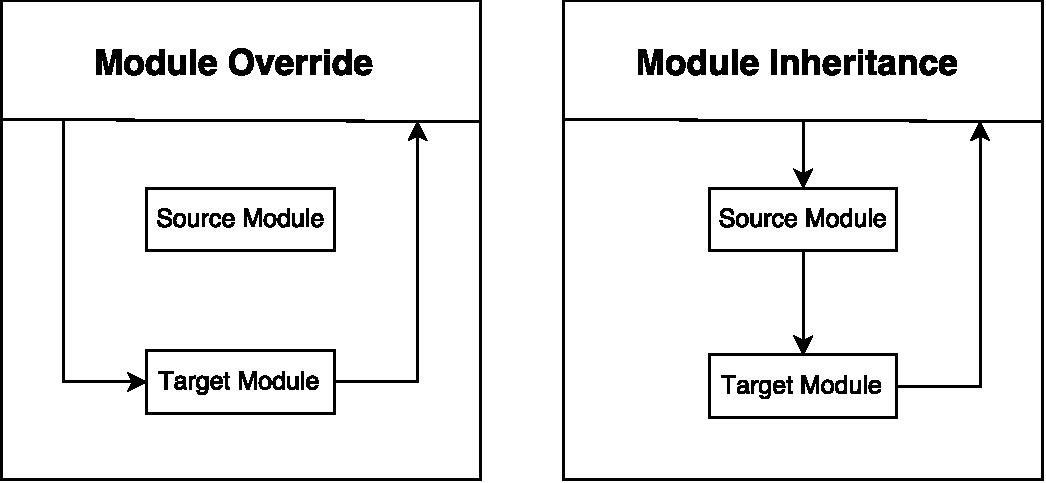
\includegraphics[width=.7\textwidth]{figs/module_hierarchy.pdf}
    \caption{Иерархия модулей}
    \label{fig:met:module_hierarchy}
\end{figure}

Один из способов развития такой архитектуры уже был упомянут ранее: иерархия модулей, построенная в базовых терминах объектно-ориентированного программирования\ref{fig:met:module_hierarchy}. В этой иерархии, модули могут либо перекрывать другие модули, либо расширять их посредством пост-обработки результатов вычислений базового модуля. Таким образом, модули сформируют классическое дерево, наследуясь от базового модуля и перехватывая поток данных. Пример подобной иерархии модулей представлен на рисунке \ref{fig:met:module_tree}.

\begin{figure}[H]
    \centering
    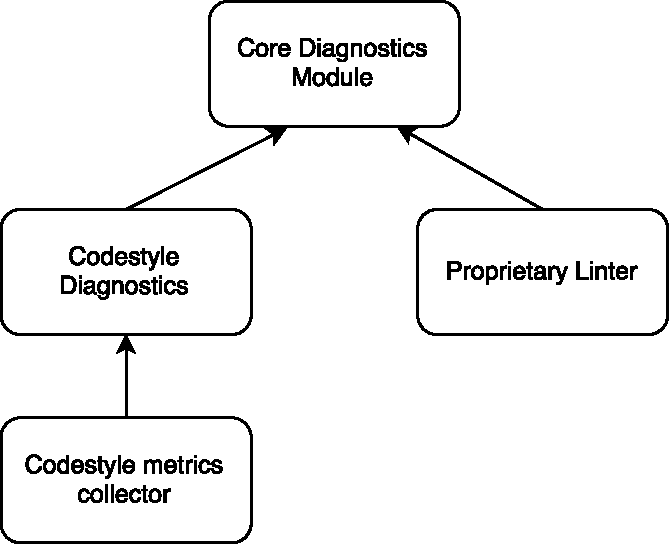
\includegraphics[width=.5\textwidth]{figs/module_tree.pdf}
    \caption{Пример дерева модулей}
    \label{fig:met:module_tree}
\end{figure}

Мы уже упомянули выше иерархию базовых и производных модулей. Взяв в качестве примера современную систему типов объектно-ориентированных языков, мы можем построить систему с базовыми модулями, которые будут доставлены пользователю в связке с самим языковым сервером и ответственны каждый за свой метод протокола ЯС. Эти модули будут главным образом предоставлять необходимый базис для всех производных модулей:
\begin{itemize}
    \item Настройка системы типов: входные данные, контекст анализа и результаты.
    \item Конструирование контекста (если применимо).
    \item Перехват результатов анализа производного модуля и отправка их клиенту через LSP.
\end{itemize}

Как можно было заметить, это не совсем классическая модель наследования объектно-ориентированной парадигмы: базовые модули не позволяют производным перекрывать свою логику, поскольку они работают с клиентом языкового сервера, и соответственно остаются запущенными внутри того же процесса, что и языковой сервер, в силу общего доступа к ресурсам. Процесс работы модульного языкового сервера показан на диаграмме последовательности \ref{fig:met:modules_sd}.

Соответственно, мы имеем два типа модулей:
\begin{itemize}
    \item Основные модули: встроены в процесс ЯС, предоставляют API для внешних модулей, не могут быть перекрыты.
    \item Внешние модули: прикрепляемы по необходимости, производные от основных модулей, могут быть перекрыты.
\end{itemize}

\begin{figure}[H]
    \centering
    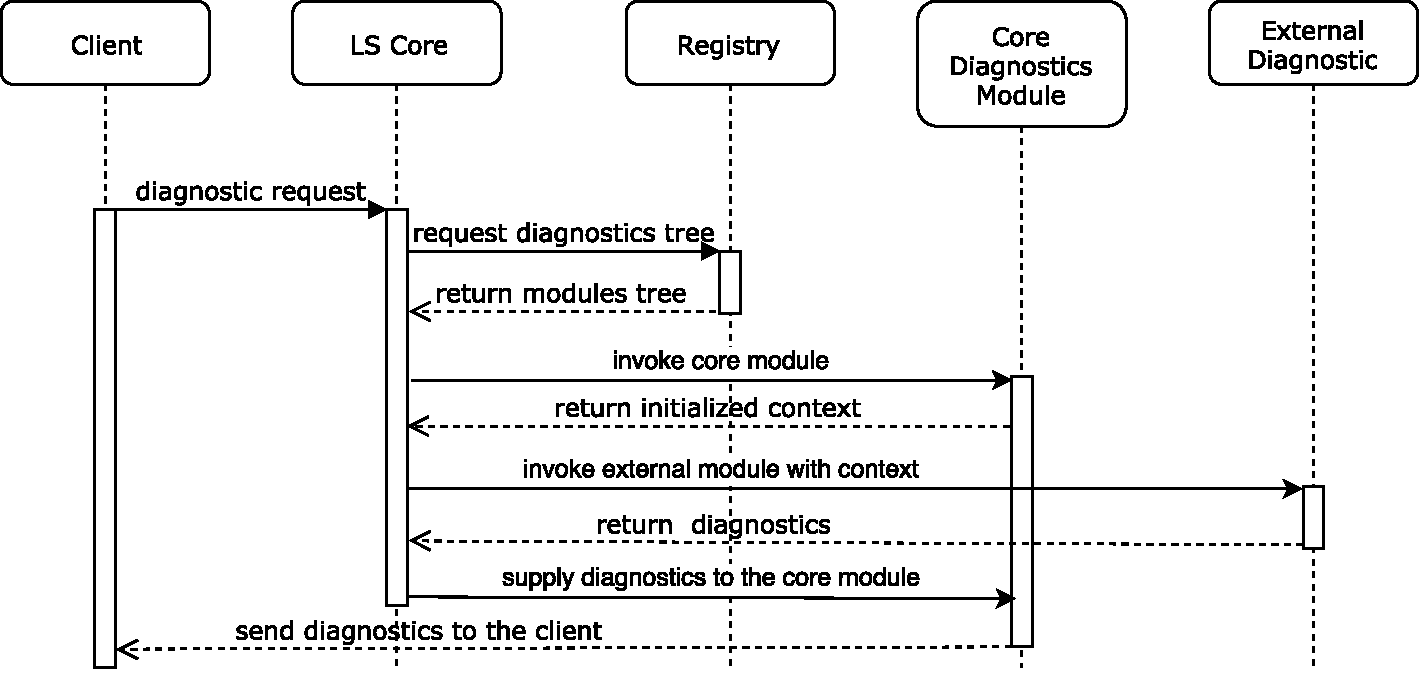
\includegraphics[width=1.0\textwidth]{figs/modules_sd.pdf}
    \caption{Диаграмма последовательности вызова модулей}
    \label{fig:met:modules_sd}
\end{figure}

Подводя итог, мы нашли способ интегрировать компилятор в языковой сервер, реализовать мощную расширяемую архитектуру, позволяющую включать дополнительный функционал для языкового сервера и иерархию модулей, и соответственно можем начать разрабатывать базовые модули для методов протокола языкового сервера, а также внешние модули для произведения анализа и трансляции ценных фактов об исходном коде клиентам языкового сервера.